\subsection{PC Next stage}
The PC next stage is in principle the fetch stage as introduced in our curriculum 
\cite{curriculum}, except the instruction memory which in our implementation is located
outside of the CPU. This stage is responsible for keeping the current PC aswell as 
calculating the next PC.

We ran into some problems when we initially used a separate PC register that clocked 
in the next PC on rising edge. The source of the problem was the instruction memory.
As it has a synchronous read and latches that read address on rising clock edge,
what happend was that the address the instruction memory had latched in lagged one step
behind what was in the PC register. When we implemented
stall this caused a real problem, as a stall caused the PC register to stop, but the
instruction memory lagged on behind it and caught up on the next rising edge, resulting in loss of one instruction.

In order to solve this we made a slight edit in the memory implementation, adding a new output singal that sends out the current clocked-in read address value. 
We use this output as our PC value, and the read address input is connected to a mux
that selects the next PC value. In essence we use the memory file as our PC register.

The PC stage takes two inputs related to jumping, a jump address and a flag indicating
a jump. Despite the name the jump inputs does not necessarily represent a jump, it may
also be a branch, but in the eyes of the PC next stage these two are equivalent.

\begin{figure}[h]
        \centering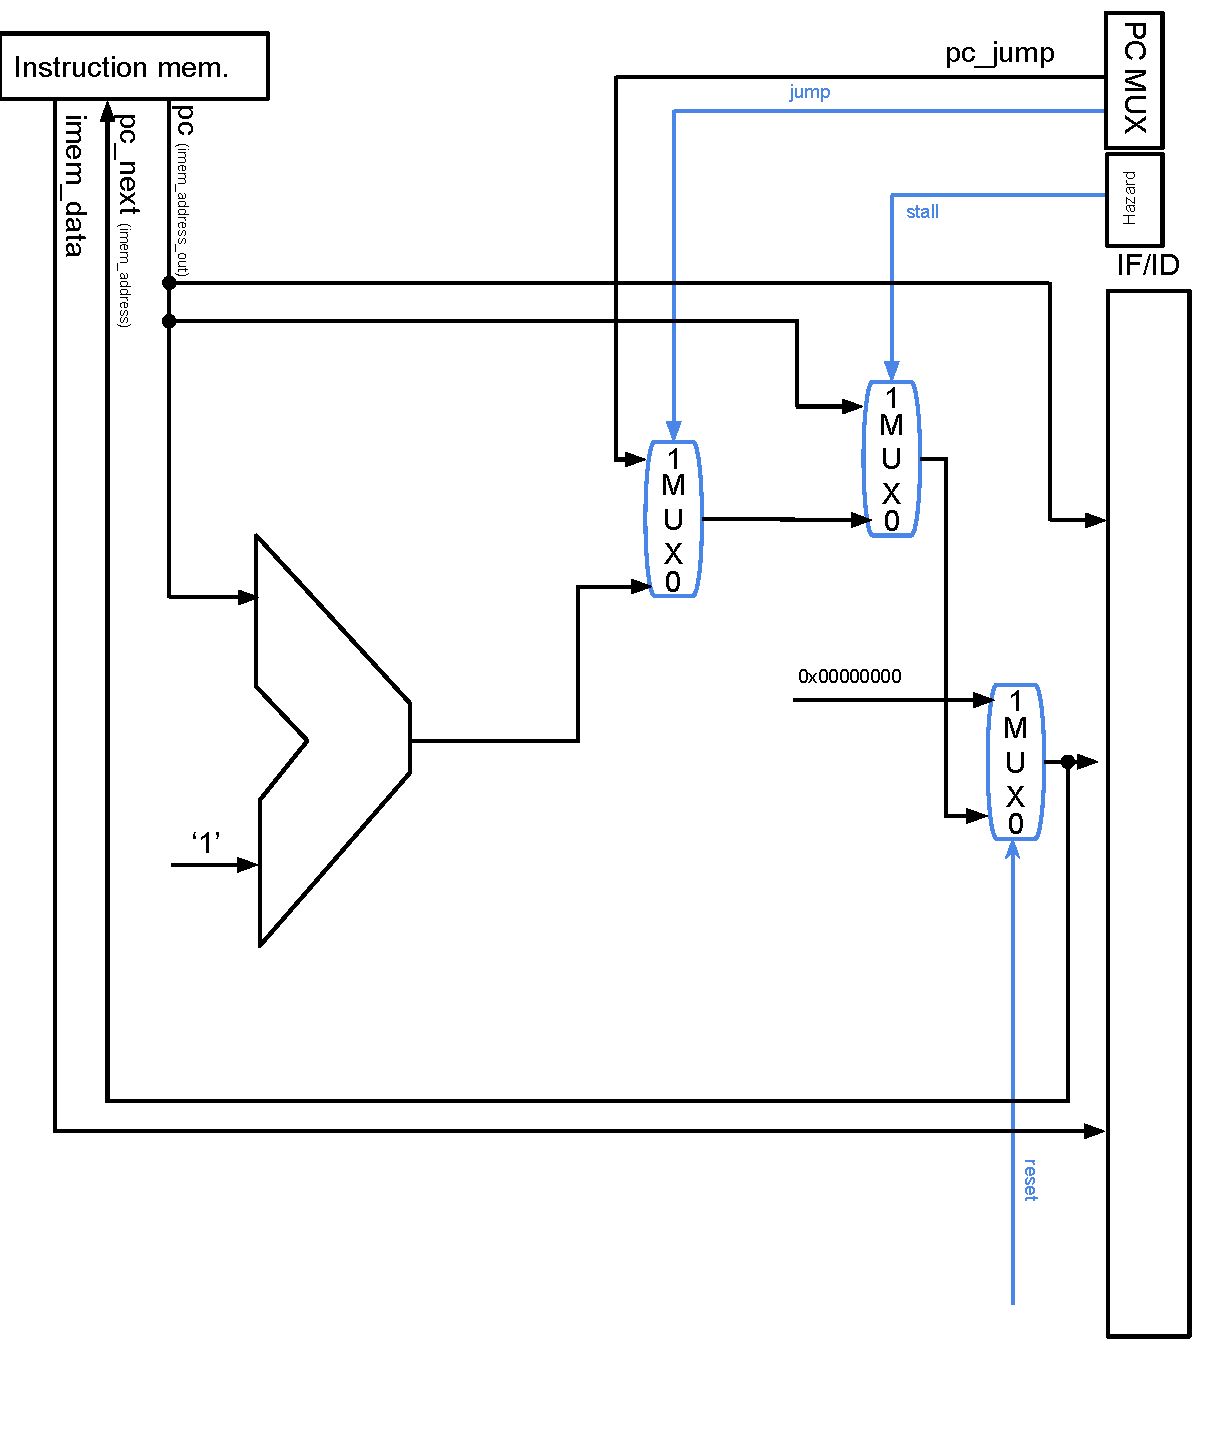
\includegraphics[scale=0.5]{figures/stage_pc_next}
        \caption{The stage\_pc\_next architecture}
        \label{fig:stage_pc_next}
\end{figure}

Figure~\ref{fig:stage_pc_next} shows a detailed overview of the architecture of the 
pc next stage. In addition to what has already been explained it can be seen that 
stalling of this stage is implemented by a mux that loops the current PC back into
the read address. Reset has also been implemeneted and it will cause the PC to reset
to the first address.